% This file is isea.tex.  It contains the formatting instructions for and acts as a template for submissions to ISEA 2015.  It is based on the ICCC  formats and instructions.  It uses the files isea.sty, isea.bst and isea.bib, the first two of which also borrow from AAAI IJCAI formats and instructions.
% Modified from ICCC.tex by B. Bogart

\documentclass[letterpaper]{article}
\usepackage{isea}
\usepackage[pdftex]{graphicx}
\usepackage{times}
\usepackage{helvet}
\usepackage{courier}
\usepackage{svg}
\usepackage[numbers]{natbib}
\pdfinfo{
  /Title (Distributed Switch Architecture, A.K.A. DSA)
  /Author (Andrew Lunn, Vivien Didelot, Florian Fainelli)}
% The file isea.sty is the style file for ISEA 2015 proceedings.
%
\title{Distributed Switch Architecture,\\ A.K.A. DSA}
\author{1\textsuperscript{st} Andrew Lunn, 2\textsuperscript{nd} Vivien Didelot,  3\textsuperscript{th} Florian Fainelli\\
  \\
  \textsuperscript{1}andrew@lunn.ch,
  \textsuperscript{2}vivien.didelot@savoirfairelinux.com,
  \textsuperscript{3}f.fainelli@gmail.com\\
}
\setcounter{secnumdepth}{0}

\begin{document}
\maketitle
\begin{abstract}

  The Distributed Switch Architecture was first introduced to Linux
  nearly 10 years ago. After being mostly quiet for 6 years, it
  recently became actively worked on again by a group of tenacious
  contributors.

  In this paper, we will cover its design goals and paradigms and why
  they make it a good fit for supporting small home/office routers and
  switches. We will also cover the work that was done over the past 4
  years, the relationship with switchdev and the networking stack, and
  finally give a heads-up on the upcoming developments to be expected.
\end{abstract}

\section{Keywords}

DSA, Distributed Switch Architecture, Linux kernel network stack, SOHO
switches, switchdev.

\section{Introduction}

Distributed Switch Architecture is a Marvell SOHO switch
term. However, as is often the case with the Linux Kernel, the code to
support it has been generalised, and now supports a number of
different vendors Ethernet switches.

The basic hardware configuration for DSA is shown in Figure
\ref{dsa-basic}. The Ethernet switch has one port dedicated to passing
Ethernet frames to/from the CPU, port 8 in the figure. This port is
connected to an Ethernet controller of the CPU acting as the
management interface. The CPU's Ethernet controller is referred to as
the 'master' interface, while the switch port is referred to as the
'cpu' port. The remaining switch ports are user ports. DSA provides a
Linux network interface for these user ports, known as 'slave'
interfaces. The slave interfaces are standard Linux network
inferfaces, as shown in figure \ref{network-interfaces}, from the ZII
devel B board.  \verb|eth1| is the 'master' interface, and the 'slave'
interfaces are \verb|lan*| and \verb|optical*|.

Overall, this forms the data plane.

\begin{figure}[ht]
  \centering
  \includegraphics[width=\columnwidth]{DSA-basic.eps}
  \caption{The Basic DSA setup}
  \label{dsa-basic}
\end{figure}

\begin{figure*}
  \begin{minipage}{\textwidth}
    \tiny
\begin{verbatim}
# ip link show
1: lo: <LOOPBACK,UP,LOWER_UP> mtu 65536 qdisc noqueue state UNKNOWN mode DEFAULT group default qlen 1000
    link/loopback 00:00:00:00:00:00 brd 00:00:00:00:00:00
2: eth0: <BROADCAST,MULTICAST,UP,LOWER_UP> mtu 1500 qdisc pfifo_fast state UP mode DEFAULT group default qlen 1000
    link/ether ec:fa:aa:01:12:fe brd ff:ff:ff:ff:ff:ff
3: eth1: <BROADCAST,MULTICAST,UP,LOWER_UP> mtu 1500 qdisc pfifo_fast state UP mode DEFAULT group default qlen 1000
    link/ether 06:34:73:83:15:6b brd ff:ff:ff:ff:ff:ff
4: lan0@eth1: <BROADCAST,MULTICAST> mtu 1500 qdisc noqueue state DOWN mode DEFAULT group default qlen 1000
    link/ether 06:34:73:83:15:6b brd ff:ff:ff:ff:ff:ff
5: lan1@eth1: <BROADCAST,MULTICAST> mtu 1500 qdisc noqueue state DOWN mode DEFAULT group default qlen 1000
    link/ether 06:34:73:83:15:6b brd ff:ff:ff:ff:ff:ff
6: lan2@eth1: <BROADCAST,MULTICAST> mtu 1500 qdisc noqueue state DOWN mode DEFAULT group default qlen 1000
    link/ether ce:00:11:22:33:44 brd ff:ff:ff:ff:ff:ff
7: lan3@eth1: <BROADCAST,MULTICAST> mtu 1500 qdisc noqueue state DOWN mode DEFAULT group default qlen 1000
    link/ether 06:34:73:83:15:6b brd ff:ff:ff:ff:ff:ff
8: lan4@eth1: <BROADCAST,MULTICAST> mtu 1500 qdisc noqueue state DOWN mode DEFAULT group default qlen 1000
    link/ether 06:34:73:83:15:6b brd ff:ff:ff:ff:ff:ff
9: lan5@eth1: <BROADCAST,MULTICAST,UP,LOWER_UP> mtu 1500 qdisc noqueue state UP mode DEFAULT group default qlen 1000
    link/ether 06:34:73:83:15:6b brd ff:ff:ff:ff:ff:ff
10: lan6@eth1: <BROADCAST,MULTICAST> mtu 1500 qdisc noqueue state DOWN mode DEFAULT group default qlen 1000
    link/ether 06:34:73:83:15:6b brd ff:ff:ff:ff:ff:ff
11: lan7@eth1: <BROADCAST,MULTICAST> mtu 1500 qdisc noqueue state DOWN mode DEFAULT group default qlen 1000
    link/ether 06:34:73:83:15:6b brd ff:ff:ff:ff:ff:ff
12: lan8@eth1: <BROADCAST,MULTICAST> mtu 1500 qdisc noqueue state DOWN mode DEFAULT group default qlen 1000
    link/ether 06:34:73:83:15:6b brd ff:ff:ff:ff:ff:ff
13: optical3@eth1: <BROADCAST,MULTICAST,UP,LOWER_UP> mtu 1500 qdisc noqueue state UP mode DEFAULT group default qlen 1000
    link/ether 06:34:73:83:15:6b brd ff:ff:ff:ff:ff:ff
14: optical4@eth1: <NO-CARRIER,BROADCAST,MULTICAST,UP> mtu 1500 qdisc noqueue state LOWERLAYERDOWN mode DEFAULT group default qlen 1000
    link/ether 06:34:73:83:15:6b brd ff:ff:ff:ff:ff:ff
\end{verbatim}
  \end{minipage}
  \caption{Standard and DSA Network interfaces}
  \label{network-interfaces}
\end{figure*}


The Ethernet switch is also connected to the CPU via a management
interface. Often this is MDIO, but can also be I2C, SPI, or memory
mapped. The management interface is used to configure the switch,
retrieve status and access statistics counters.

Ports 0 to 2 of the switch connect directly to RJ45 connectors. In
this case, the Ethernet PHY is embedded within the switch, and managed
via the switch management interface. Typically this is achieved via
the switch having an internal MDIO bus, and exporting registers to
control this MDIO bus. The DSA software framework exports this MDIO
bus to Linux as a normal MDIO bus. Thus the PHYs on the bus can be
probed, the existing Linux PHY drivers used, and the PHYs associated
to the Linux slave interfaces representing the switch ports.

Port 3 shows a Fiber interface. Typically this is controlled and
monitored via I2C, and would be connected to the hosts I2C
controller. Again, this Fiber module is associated to the slave
interface and can be managed using standard Linux tools.

Lastly, ports 4 and 5 use external PHYs, connected via RGMII to the
switch. Either the PHYs are managed via the switches own MDIO bus, as
used by the internal PHYs, or they can be connected to the CPUs MDIO
bus. As with the internal PHYs, Linux can manage the external PHYs and
associate them to the Linux slave interface representing the switch
ports.

Overall, this forms the control plane.

DSA is however not limited to a single switch. Figure \ref{d-in-dsa}
shows an architecture of multiple switches connected together. This is
the D in DSA, a distributed switch fabric. Currently, Linux only supports
Marvell switches in this configuration, however the concept is
generic, so other switch vendors featuring cascaded switches should be
supportable.

\begin{figure}[ht]
  \centering
  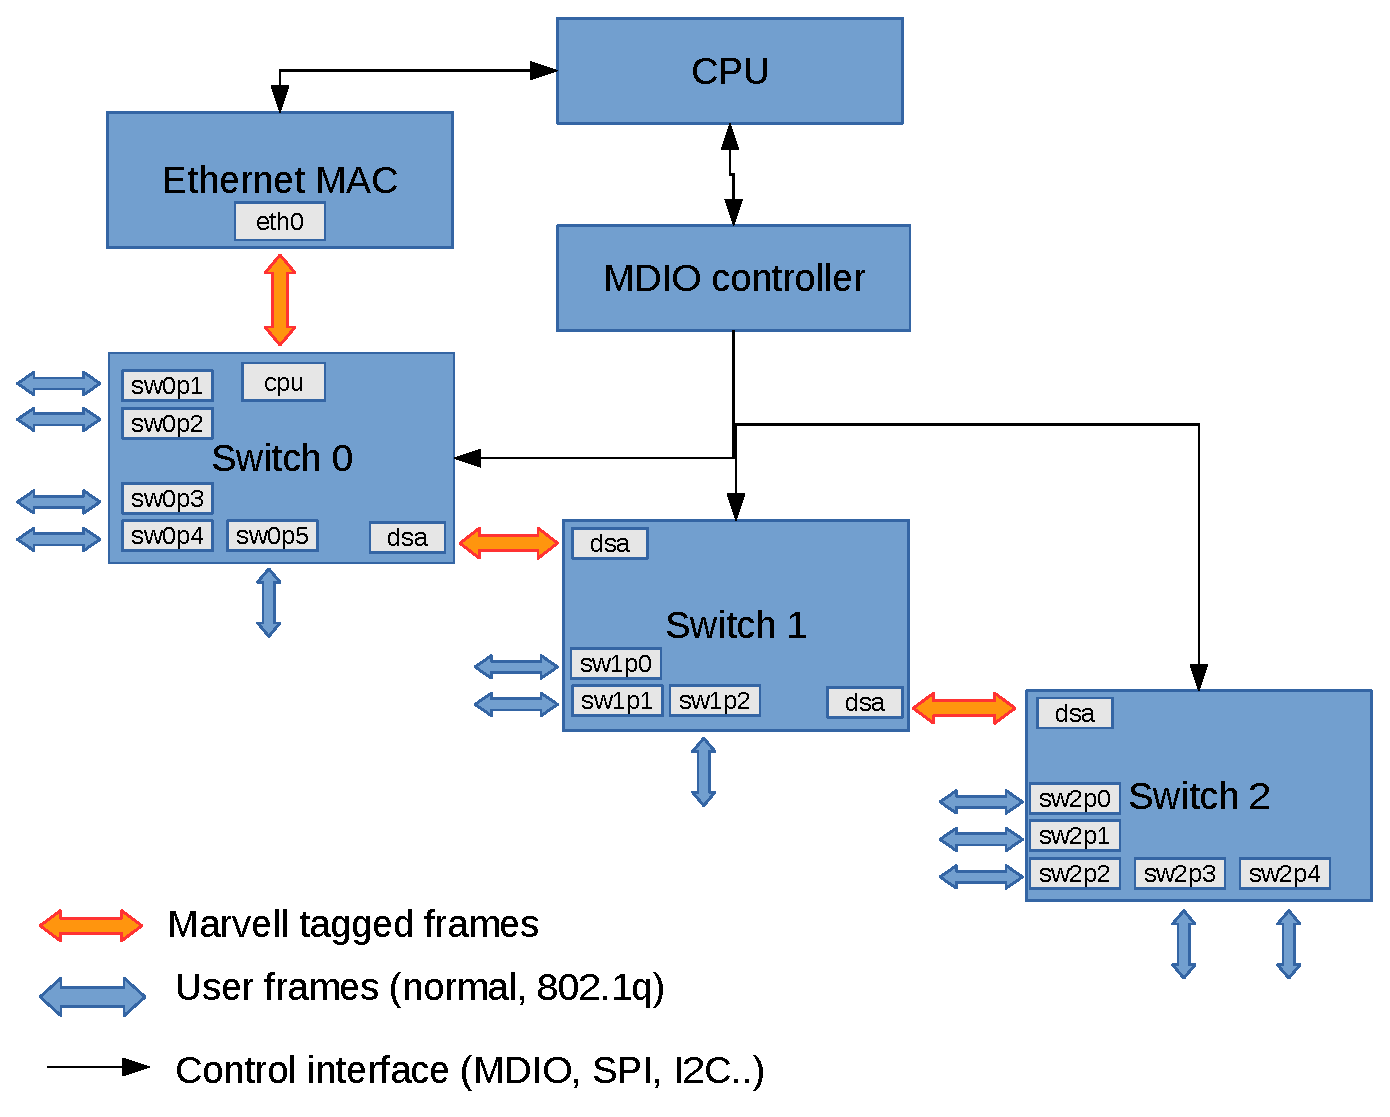
\includegraphics[width=\columnwidth]{DSA-D-in-DSA.eps}
  \caption{The D in DSA setup}
  \label{d-in-dsa}
\end{figure}

Again, one switch is connected to the CPU via an Ethernet controller
to form the data plane between the CPU and the switches. This port is
referred to as the 'cpu' port. And there is a management plane via
MDIO, or SPI, I2C, MMIO. However, the data plane is extended to the
cascaded switches via the 'dsa' ports. These ports are used to connect
switches together, so that frames can be passed between switches, or
forwarded to the CPU via its Ethernet controller. The management plane
is extended, in that each switch is connected to the management plane.
Note that 'dsa' ports are not visible to the user as normal network
devices.

The distributed nature of the switch is hidden from the user. Only a
collection of Linux network interfaces are seen. Figure
\ref{network-interfaces} illustrates this, in that the board actually
has three switches.

The key concept for DSA, which differentiates DSA from pure switchdev
supported switches is a port connected to an Ethernet controller to
form the data plane. Later sections describe this, and the
relationship between DSA and switchdev, in more detail. In contrast,
on top-of-the rack switches that switchdev typically supports, each
switch port may have its own DMA-capable Ethernet MAC to send/receive
frames to/from the CPU acting as a management interface.

\section{User of DSA}

Users of DSA fall into two main categories.

\subsection{WiFi Access Points/Routers and Set-Top Boxes}

Probably the most obvious use of DSA is in set-top boxes, and WiFi
access points/routers. These typically have 5 Ethernet ports on the
back, often labeled WAN and LAN 1-4. Figure \ref{wrn854t} is an
annotated image of the Netgear WNR854T, which contains a Marvell 8
Port Ethernet switch. Figure \ref{BCM97445VMS} is a BCM97445VMS board
with an external BCM53125 switch at the top-left with a 4-RJ45
connector.

\begin{figure}[ht]
  \centering
  \includegraphics[width=\columnwidth]{wnr854t_board_annotated}
  \caption{Annotated WRN854T WiFi Access Point, image from OpenWrt}
  \label{wrn854t}
\end{figure}

\begin{figure}[ht]
  \centering
  \includegraphics[width=\columnwidth]{20170329_174239}
  \caption{Broadcom BCM97445VMS Board with an BCM53125 Switch at the top-left}
  \label{BCM97445VMS}
\end{figure}

\subsection{Industrial Switches/Routers}

There have been a number of contributions to DSA drivers from
industrial switch/router vendors from the transport industry. DSA has
been flying in aircraft inflight entertainment (IFE) systems for a
number of years. Busses and trains are becoming more networked, in
order to provide passenger information systems, with DSA being used in
the network equipment. Figures \ref{netmodules} and \ref{ife} show a
couple of example devices.

\begin{figure}[ht]
  \centering
  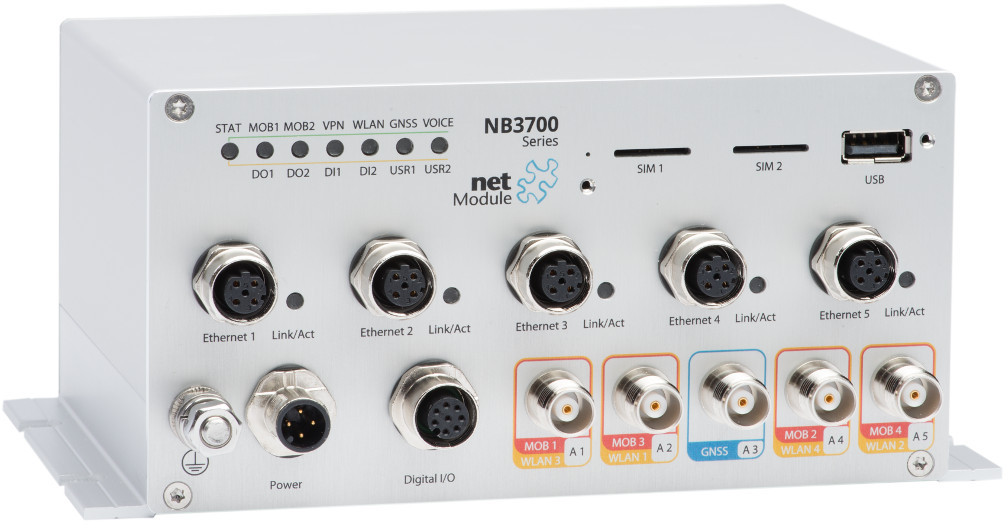
\includegraphics[width=\columnwidth]{netmodules}
  \caption{Netmodules transport router}
  \label{netmodules}
\end{figure}

\begin{figure}[ht]
  \centering
  \includegraphics[width=\columnwidth]{IMG_20170302_080726}
  \caption{IFE aircraft switch}
  \label{ife}
\end{figure}

\section{History}

DSA is not a new subsystem in the Linux kernel. It was added in 2008,
with support for a limited number of Marvell SOHO switches (Linkstreet
product line). However, after the initial contribution, development
was dormant, as can be seen in Figure \ref{dsa-activity}, which shows
the number of lines changed per month, between 2008 and the end of
2016.

\begin{figure}[ht]
  \centering
  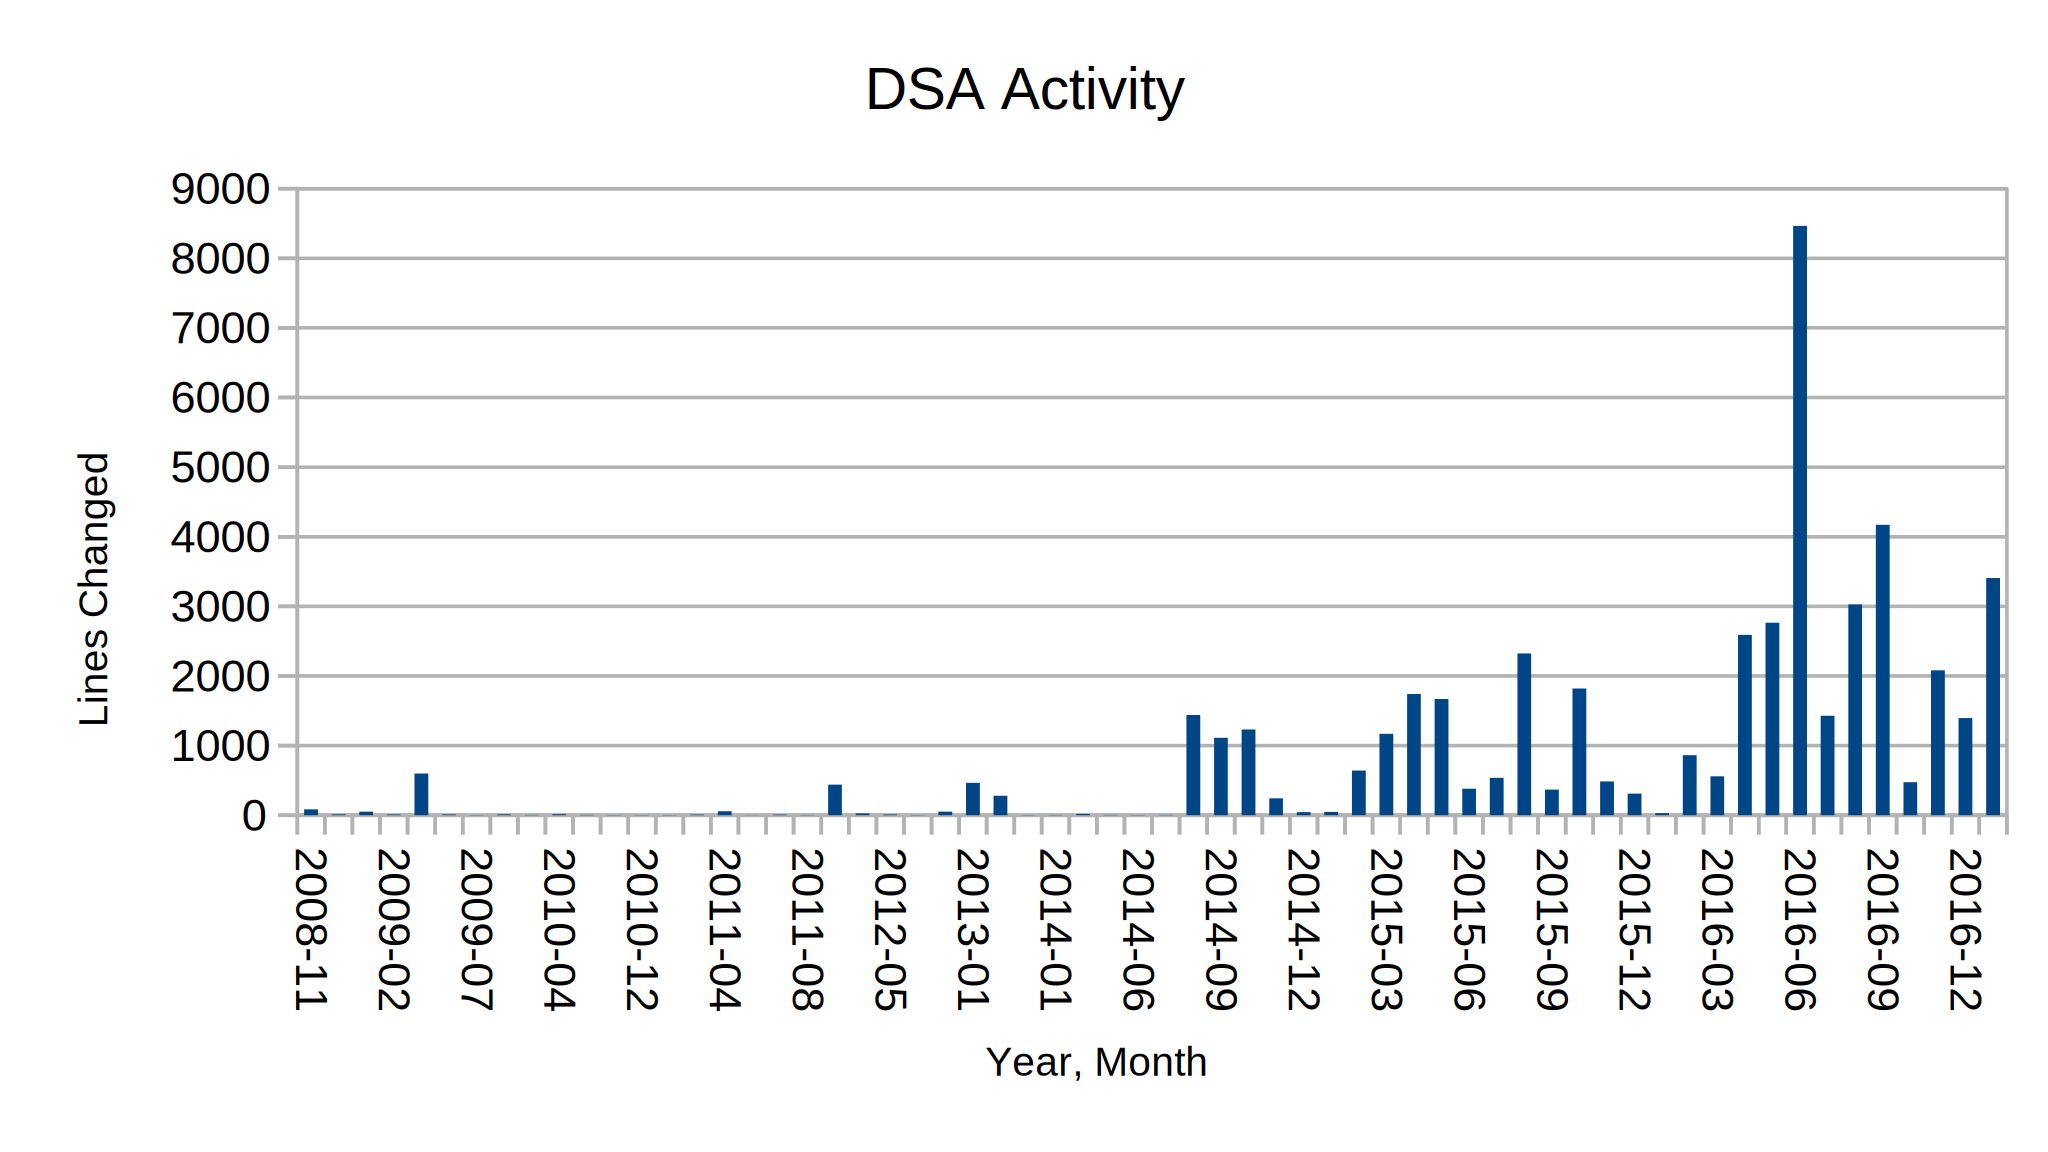
\includegraphics[width=\columnwidth]{dsa-activity}
  \caption{DSA development activity, in terms of lines changed per
    month}
  \label{dsa-activity}
\end{figure}

From 2008 to the middle of 2014, the changes are those typical for
maintenance churn, caused by changing internal kernel APIs. No new
features or devices were added during this time.

From the end of 2014, development recommenced, as part of the Linux
networking push to support hardware offloads and network switches. In
2014 Broadcom added support for their Starfighter 2 switch. Often
switches features can be configured via an EEPROM. Linux network
interfaces already support this concept, and it was extended to
support access to switch EEPROMs. Some switches contain temperature
sensors, so infrastructure was added to export these sensors via the
HWMON subsystem. Modern switches implement Energy Efficient Ethernet,
a mechanism to save power on idle interfaces. The extending kernel
support was extended to switch ports. Wake-on-LAN support was also
added, following the standard abstractions. As described in the
introduction, switch ports have Ethernet PHYs. The phylib was better
integrated into DSA. Lastly, a new Marvell family of switches, the
88E6352 was added in 2014.

Development continued in 2015 adding a device tree binding. Up until
then, only platform data could be used to describe the hardware
architecture. This was the time that ARM platforms swapped to using
device tree, and most boards using DSA are ARM based. A major new
feature was making use of the switch hardware to perform bridging
between ports. Up until then, the ports simply forwarded all frames to
the CPU, and the CPU performed bridging, if configured and
required. This was the first step in using the switch hardware as an
accelerator, not just a port multiplexer.

In 2016 the limitations of the original architecture became a major
problem for supporting switches which were not managed via
MDIO. Refactoring work was performed to represent switches as Linux
devices, and to abstract out the communication mechanism used to the
switch. It then became possible to use SPI, I2C, or MMIO for the
control plane. As a result, a new device tree binding was needed. This
refactoring opened up a path for the Broadcom B53 driver, which drives
devices using SPI and MMIO. 2016 also sore the addition of a driver
for the Qualcom QCA8K switch, and a further Marvell switch family, the
88E6240.

Development work has continued in 2017, with another Marvell switch
family, the 88E6390, the second generation Starfighter 2, and
initial contributions for the Mediatek MT7623. Additionally, more
acceleration support is being added with the support for port
mirroring and some TC offloads.

As the history as shown, DSA tries to make use of the existing kernel
abstractions and infrastructure where possible.

\section{Alternative Approaches}

Despite its long history in the kernel, DSA is not the only way to
manage Ethernet switches in WiFi access points and STBs. A number of
other solutions have been deployed in a wide range of products.

\subsection{swconfig}

OpenWrt/LEDE has an alternative solution, known as swconfig.

DSA makes use of additional tagging headers in order to direct frames
in/out of specific ports of the switch. swconfig instead uses VLAN
tags for traffic segregation. This allows swconfig to support a wider
range of switches, since most switches support VLANs, however fewer
switches support tagging headers. At the time swconfig was developed,
DSA was incorrectly considered to be a Marvell only solution and
limited to an MDIO control plane. swconfig does not have such
restrictions. Note that since then, it has also been identified that
DSA could utilize VLAN tags as the most basic form of traffic
segregation in case a switch does not support additional tagging.

The swconfig solution does not make use of the Linux network interface
abstraction. The ports of the switch are not represented as network
interfaces. This goes against the communities decision that switch
ports should be seen as standard Linux interfaces. However, it can be
argued for the OpenWrt/LEDE use cases, this not so important. WiFi
access points typically just want to bridge all the ports. There are
few use cases for using the ports individually.

swconfig uses a generic netlink based configuration mechanism, with a
base set of options and then device specific extensions. These
extensions have however resulted in inconsistency across device
drivers. Most often this inconsistency is not noticeable to the
end-user because the configuration of devices is already abstracted in
OpenWrt/LEDE thanks to UCI (Universal Configuration Interface). This
abstraction would take a standard syntax and transform it into
appropriate swconfig calls towards the specific switch driver.

swconfig was proposed \cite{swconfig} as a solution for mainline in
2013. The discussion around it and its rejection was one of the
starting points to the development of the switchdev framework.

There are a number of other of solutions, none of which should get
anywhere near mainline.

\begin{itemize}
\item SoC Vendors have hacked together quick-n-dirty /proc, /sys/,
  debugfs or ioctl() APIs for configuring switches.
\item Vendor specific and proprietary switch SDKs run in userspace,
  with a small kernel driver to export register access.
\item The bootloader configures the switch and it is never touched again!
\end{itemize}

\section{The Switch as a Hardware Accelerator}

When swconfig was rejected, there was a number of different ideas how
Ethernet switches, and other network accelerators should be modeled.
In 2014, during a number of conference corridor side discussions, the
current solution was decided upon. The solution is simple: keep the
standard Linux network interface abstractions. The consequences of
this decision can be summarized in a few points:

\begin{itemize}
\item Switch ports are modeled as Linux network Interfaces.
\item Confusing to some, switch ports don't switch traffic by default.
\item Standard Linux tools are used to configure these interfaces, e.g. ip(8) and ifconfig(8).
\item The Linux bridge abstraction is used for bridging interfaces, e.g. ip(8), bridge(8) and brctrl(8).
\item Linux team/bonding abstraction used for trunking switch ports.
\item Ethernet PHYs on switch ports are normal Linux PHYs.
\item Port statistics follow the normal abstraction provided by ethtool(8).
\end{itemize}

As a result, we use the switch hardware to accelerate what Linux can
already do with a collection of software interfaces.

\section{The Data Plane}

The data plane deals with getting Ethernet frames to/from Linux in/out
of the ports of the switch. And it is required that frames can be
addressed to specific ports, even when the ports are bridged together.
E.g. Bridge PDUs must go out specific ports of the bridge.

The majority of this code in the data plane is generic, independent of
the switch being used.

\begin{figure}[ht]
  \centering
  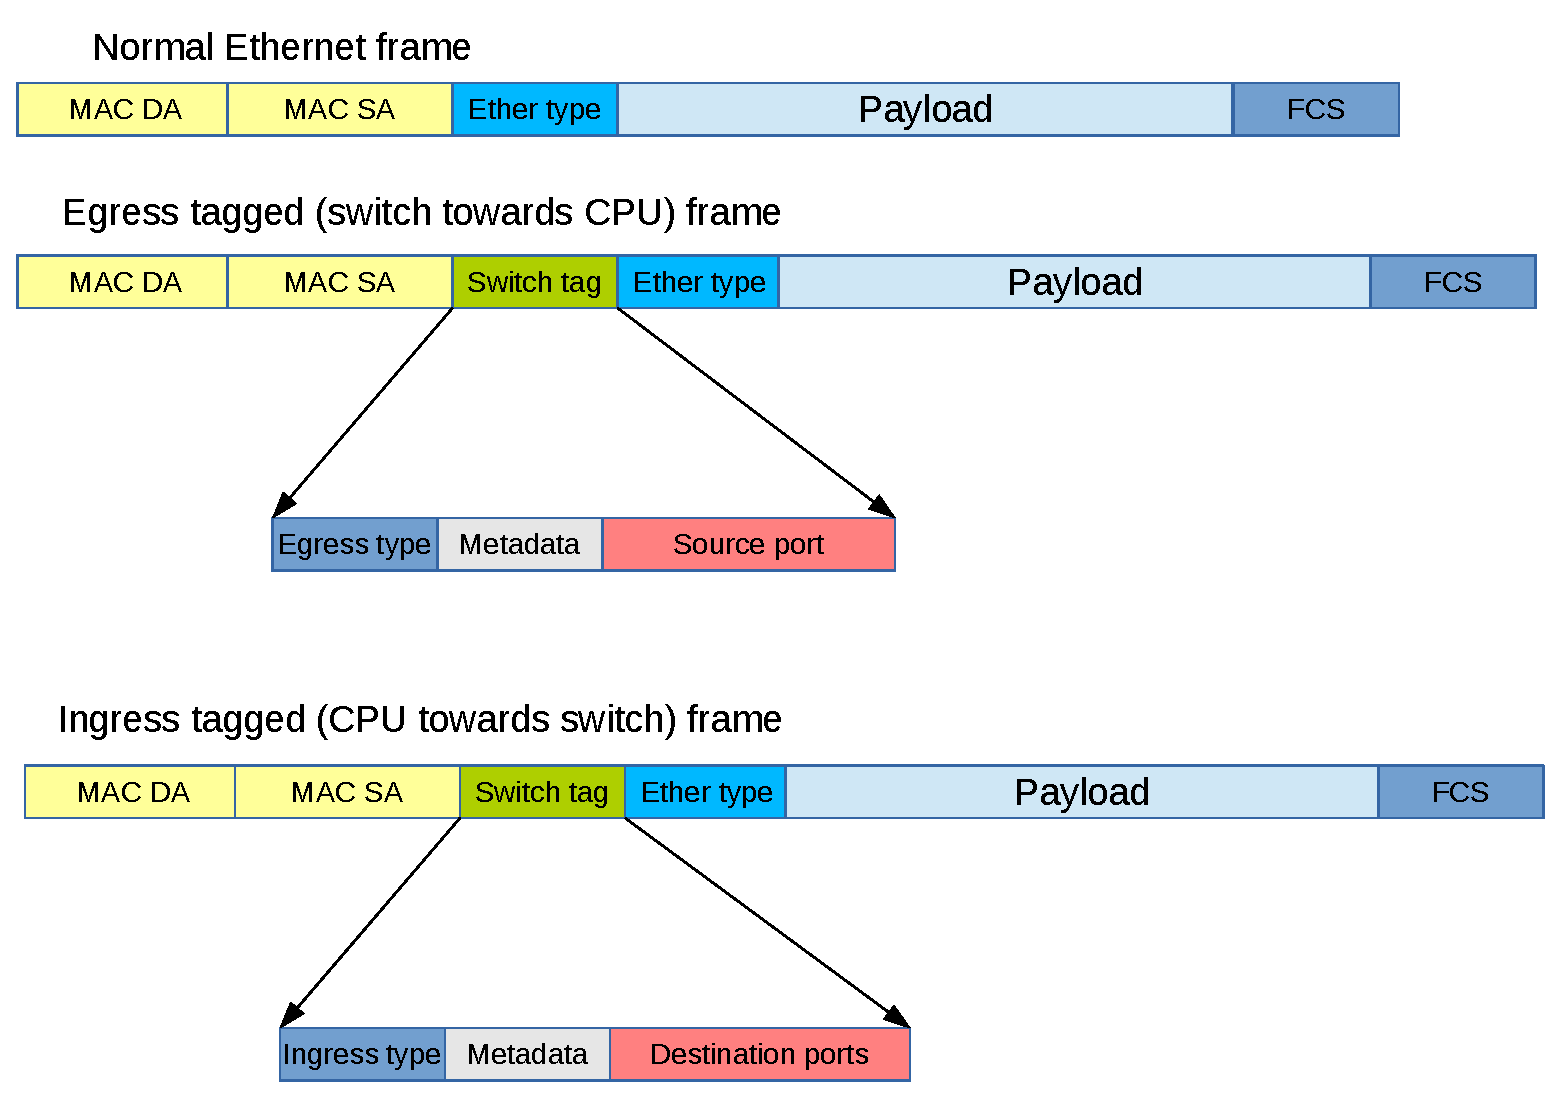
\includegraphics[width=\columnwidth]{DSA-frame-processing.eps}
  \caption{DSA Switch Tags}
  \label{DSA-frame-processing}
\end{figure}

Frames sent from the CPU to the switch are tagged with an additional
header, as shown in figure \ref{DSA-frame-processing}. The top frame
in the figure is that passed to a slave interface by the Linux network
stack. The bottom frame is that which egresses the master interface,
the CPU network controller, and ingresses to the switch. The switch
tag, which is generally added after the source MAC address, is used to
direct the frame out a specific vector of ports of the switch.
Additionally, when there are multiple switches, it indicates which
switch the egress port belongs to. The tag indicates if this is an
ingress or egress frame, relative to the switch. The metadata varies
between tagging protocols, but can for example indicate the presence
of a VLAN tag within the switch tag, the CFI, or the frame priority.

Frames which egress the switch to the CPU Ethernet controller have a
similar switch tag. The metadata may indicate why the switch egressed
the frame to the CPU. The source port indicates the ingress port of
the switch, and when there are multiple switches, which switch the
ingress port belongs to.

Figure \ref{wireshark} shows a wireshark dissection of an Ethernet
frame with a Marvell EDSA tag. The NTP frame is being sent by the CPU
to egress port 3 of switch 0.

\begin{figure}[ht]
  \centering
  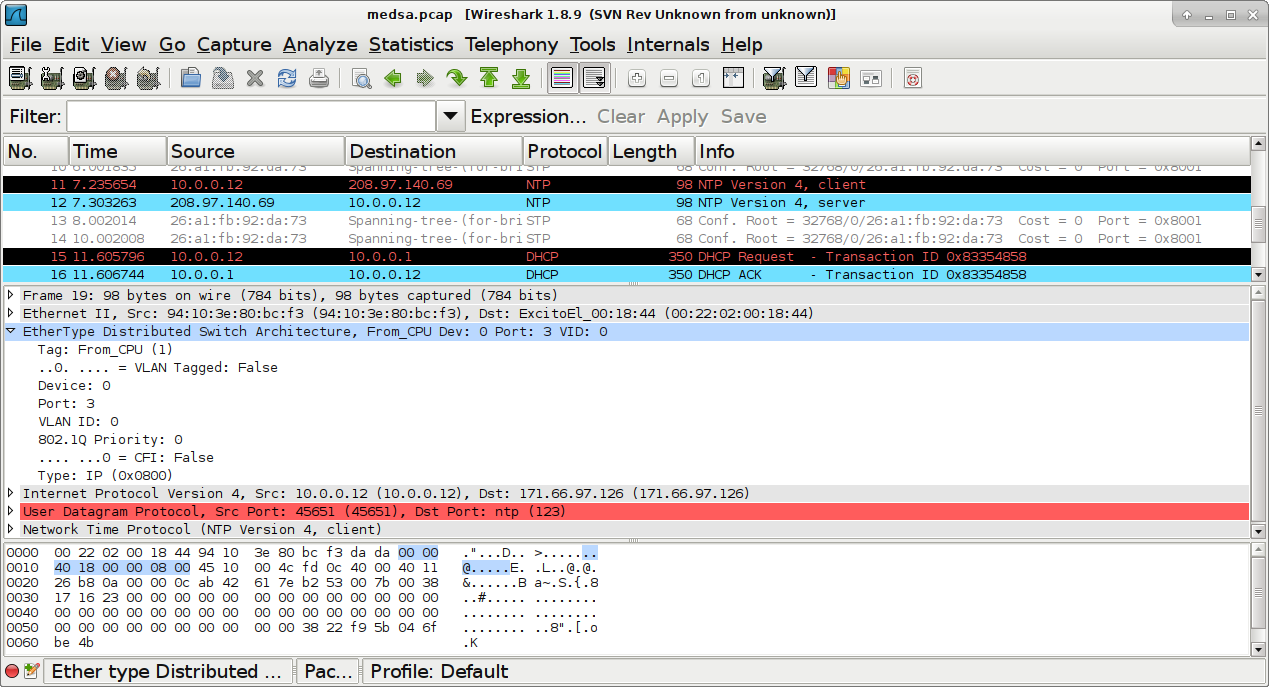
\includegraphics[width=\columnwidth]{wireshark}
  \caption{Marvell ESDA tag shown in Wireshark}
  \label{wireshark}
\end{figure}

DSA has a number of protocol taggers to insert/remove the switch
tags. Currently there are taggers for Marvell DSA and EDSA, Broadcom,
Qualcom, and the Mediatek tagger is under review.

Figure \ref{stackflow} shows how these tagging protocols are used.

\begin{figure}[ht]
  \centering
  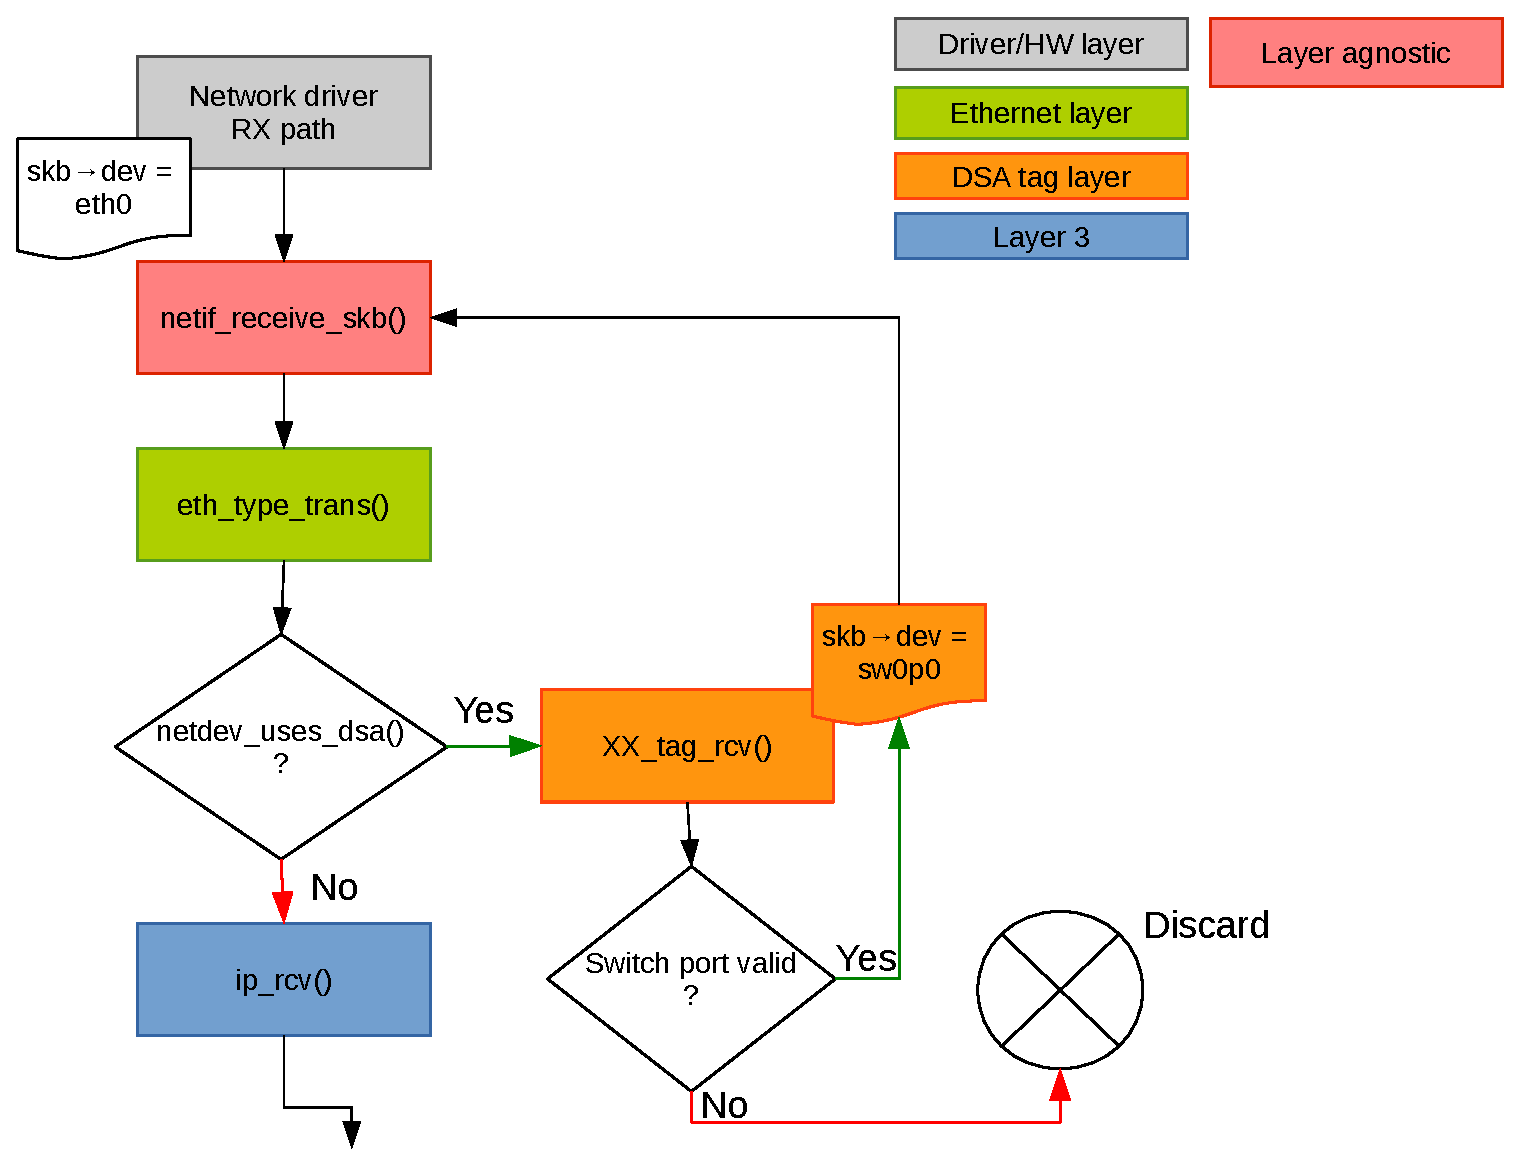
\includegraphics[width=\columnwidth]{dsa_explained.eps}
  \caption{Processing the Switch Tag}
  \label{stackflow}
\end{figure}

The frame from the switch is received by the CPU's Ethernet controller,
and the driver calls \verb|netif_receive_skb()| to pass the frame to
the network stack in the normal way. \verb|eth_type_trans()| is called
to determine the Ether Type of the frame. As part of
\verb|eth_type_trans()|, a check is made to see if the ingress
interface is a DSA master interface, i.e. \verb|netdev_uses_dsa()|. If
so, tagged frames are expected. The tag protocol receiver function is
then invoked on the frame. This extracts the information from the tag,
and then removes the tag from the frame. If the switch ingress port is
valid, the DSA slave interface is determined, and the ingress
interface is updated in the \verb|skb| to point to the slave
device. The frame is then again passed to the network stack using
\verb|netif_receive_skb()|. This time the true Ether Type can be
extracted from the frame, and the frame is passed on for IP
processing, etc.

The transmit path is similar. The slaves transmit function invokes the
tagger transmit function. It inserts the switch tag, and then calls
the master interface's transmit function via \verb|dev_queue_xmit()|.

This way of popping or pushing the switch tag is completely standard
and uses Linux's way of dealing with a stack of devices on top of each
other.

\section{Control Plane}

The control plane for switches in the DSA framework makes use of
switchdev to interface with the Linux network stack's control plane.

\subsection{switchdev}

switchdev is a stateless framework within the kernel stack which lives
under \verb|net/switchdev|. It provides the needed control knobs
within the network stack's control plane to push tasks which can be
offloaded down to the hardware. It does this by offering a number of
\verb|switchdev_ops|, which switch-like devices can
implement. Examples of this are adding/removing a VLAN to a port,
adding/removing a forwarding database entry to a port, changing the spanning
tree protocol state of a port, etc. In order to support the diverse
ways VLANs, forwarding database entries, etc. can be represented in
hardware, switchdev provides an abstract model of these objects. It is
the responsibility of the ops implementer to translate the abstract
representation into a concrete representation needed by the switch.

switchdev is not a driver model. It does not define what a switch
is. It just defines operations that switch-like devices may
implement. This makes the API flexible to a wide range of
hardware. The main user of this API is switches, but it can also be
used with Ethernet controllers with SRIOV VF functionality, etc.

Additionally, switchdev is not involved in the data plane, only at the
control plane level.

In Summary, switchdev is an abstraction the network stack uses to
offload tasks down to the underlying hardware.

\subsection{DSA vs. switchdev in the Control Plane}

The DSA core framework lives under \verb|net/dsa|, with the device
drivers in \verb|driver/net/dsa|. Unlike switchdev, DSA maintains a
little state. However, it aims to keep as much state as possible
within the switch, not the driver. DSA provides an abstract model of a
switch. Each switch has a \verb|dsa_switch| structure to represent
it. The \verb|dsa_switch| structure contains a list of operations,
\verb|dsa_switch_ops| which can be performed on the switch. In order
to support the D in DSA, a collection of switches in a tree are
represented by a \verb|dsa_swith_tree|. And going the other way in the
hierarchy, each \verb|dsa_switch| has a number of \verb|dsa_port|
structures to represent each port of the switch.

Given the abstract model of a switch, DSA binds the switch to the
Linux network stack, by implementing the \verb|netdev_ops| and
\verb|ethtool_ops|, using the \verb|dsa_switch_ops| to call into the
switch driver. Additionally, DSA implements the \verb|switchdev_ops|
by again calling into the switch driver via \verb|dsa_switch_ops|.

DSA also provides a well defined device tree binding to describe the
switch ports, their names, their connection to an internal/external
PHY, and how they are interconnected in a D in DSA system.

In summary, DSA provides the glue between the network stack and the
switch device drivers.

\section{Future Development Work}

DSA is not complete. In fact, there is a lot left to do, when
comparing the features supported by DSA with the ones supported by switchdev
devices like the
Mellanox mlxsw \cite{mlxsw}. The bottleneck is the availability of developers
to implement these features, not the framework itself.

It is hoped the following features will appear during 2017.

\begin{itemize}
\item Merge the Mediatek driver. This driver is currently under review
  and might be merged before this paper is even presented!
\item Add support for Microchip devices. Microchip is working on a
  driver and hope to contribute it soon.
\item Multiple CPU ports. Some WiFi access points have two ports
  connected to CPU Ethernet controllers, in order to increase the
  bandwidth between the CPU and the switch. However, DSA currently is
  limited to a single CPU Ethernet controller. The vendor firmware
  configures one of the two CPU interfaces and the switch in a
  straight though manor, to implement the WAN port of the
  device. Although simple, it potentially does not make the best use
  of the available bandwidth. The tagging headers already guarantee
  traffic segregation, so there is no need to dedicate a CPU Ethernet
  controller to the WAN port. DSA will be extended to allow multiple
  CPU ports to be defined, and where possible, implement basic load
  balancing across these CPU ports. Each CPU ports will send traffic
  to a subset of the switches ports.
\item IGMP snooping. Currently, all multicast traffic is flooded to
  all interfaces with the switch. However, these switches have the
  ability to detect IGMP packets and direct them to the CPU. The Linux
  bridge already supports IGMP snooping, so feeding these IGMP packets
  to the bridge will allow the bridge to decide which interfaces
  multicast frames should egress, and which interfaces have no
  interest in the multicast frames and can be blocked. By implementing
  the needed switchdev callbacks, this knowledge can be pushed down
  into the switch to control the flooding. This is particularly
  important when the CPU is low powered, aimed at simply managing the
  switch. It has no interest in the multicast data itself, and a high
  volume of multicast traffic can overload it.
\item Better D in DSA for Marvell switches. Currently, the distributed
  part of DSA is primitive. The support for VLANs spanning multiple
  switches is limited. Bridges spanning multiple bridges may leak
  frames, etc. Work is in progress to improve this.
\item Better support for Fiber interfaces. SFP modules are being seen
  on consumer devices, and industrial routes often have SFP modules.
\item Improved automated testing using open source software (Ostinato)
  \cite{ostinato}
\end{itemize}

There are also some more long term goals.

\begin{itemize}
\item Team/Bonding support.
\item TCAM support to offload parts of the firewall.
\item Qualcom Hardware NAT.
\item Metering, broadcast storm suppression.
\item More TC support for QoS priorities and maps and other offloads.
\end{itemize}

It would also be good to have more vendor endorsed development. We are
already in a good position with 4 vendors supporting their own
devices. But there are more vendors and devices out there. It does
however seem that switch vendors are now realizing that to be part of
the Linux kernel, they have to use switchdev, and where appropriate,
DSA.

\section{Conclusions}

DSA is now a mature and working subsystem which has received support
from a fair amount of contributors actively using it in existing
products. Although there is still a long way to go in terms of feature
completeness regarding what existing Ethernet switches can do, the
fundamental paradigm that a switch port should be a Linux network
device has been proven successful.

DSA benefits from working on a product space that is today largely
mature and receives little radical changes that would require a
complete redesign.  The latest major change was in the device driver
model aspect and has since opened the door to supporting many more
devices. Having to support such devices allows developers to focus on
bringing additional features into what Linux can already do, and
therefore pushing for better integration of offloads.

Ultimately, the goals of getting a device supported in Linux is to get
finer and better control over what existing WiFi access points/routers
and other Linux based network products can do. Better control allows
building reliable, scalable and sustainable networks with equally
scalable open source solutions, benefiting every one.

\begin{thebibliography}{2}
\bibitem{swconfig}
net: phy: add Generic Netlink switch configuration API\\
\texttt{https://www.spinics.net/lists/netdev/msg254794.html}

\bibitem{mlxsw}
Mellanox Technologies Switch ASICs support\\
\texttt{https://git.kernel.org/pub/scm/linux/kernel/git/\\
  torvalds/linux.git/tree/drivers/net/ethernet/mellanox/mlxsw}

\bibitem{ostinato}
  Ostinato Network Traffic Generator\\
  \texttt{http://ostinato.org/}

\end{thebibliography}

\end{document}
